\chapter{Homogeneous Space, FRW Geometry, and the Meaning of $k$}

Let us begin exactly where the lecture begins: not with expansion, but with some simple mathematics. The connection to Einstein's equations is the destination, but Leonard Susskind very deliberately refuses to go there at once. We first need a language for homogeneous curved spaces, then a way to look out from within them, and only then can the constant \(k\) reveal its double meaning. What follows is a companion account of the fifth cosmology lecture, prepared for the course notes with curation support from LazyingArt LLC and Video2Book.

\section{Uniform Geometry and the Meaning of a Sphere}

Susskind begins by reminding us that spheres are the paradigmatic \emph{uniform} geometries. Uniform here means constant curvature: every point is like every other point. That is already the cosmological theme in miniature. Before one says anything about galaxies or expansion, one asks what kinds of large-scale spaces could be homogeneous.

The first description uses an embedding space as a crutch. A one-sphere is just a circle,
\begin{equation}
x^2+y^2=a^2,
\end{equation}
with unit case
\begin{equation}
x^2+y^2=1.
\end{equation}
A two-sphere is described in the same way, only now the crutch is three-dimensional:
\begin{equation}
x^2+y^2+z^2=a^2,
\end{equation}
and the unit two-sphere is
\begin{equation}
x^2+y^2+z^2=1.
\end{equation}
For the three-sphere one adds one more coordinate,
\begin{equation}
x^2+y^2+z^2+w^2=A^2,
\end{equation}
with unit case
\begin{equation}
x^2+y^2+z^2+w^2=1.
\end{equation}

The essential point is that these ambient coordinates are not themselves the space in which the inhabitants live. The embedding space is only a device for writing an equation. The actual geometry is the sphere itself. If a creature lives on a one-sphere, it lives on a circle; it has no access to an ``outside'' or an ``inside.'' Likewise, if space were a two-sphere or a three-sphere, the geometry of interest would be the surface itself, not the surrounding Euclidean space we used to write it down.

This distinction matters immediately when the lecture turns toward cosmology. A spherical universe means that \emph{space} is spherical. It does \emph{not} mean that spacetime is some higher-dimensional sphere with time smuggled in as one more coordinate. Time will enter later, but it enters differently.

For amusement, and to show that the pattern continues backward, the lecture briefly asks about a zero-sphere. Extrapolating the same algebraic pattern gives
\begin{equation}
x^2=1,
\end{equation}
whose solutions are the two points \(x=\pm 1\). We will not need the zero-sphere later, but it makes the recursive picture of spheres feel less accidental.

\section{Intrinsic Metrics and the Recursive Sphere Construction}

The more useful description is intrinsic. We now stop leaning on the crutch and describe the sphere in coordinates that live on the sphere itself. That is the language cosmology will actually use.

For the unit one-sphere a single angular coordinate \(\phi\), with \(0\leq \phi < 2\pi\), is enough. The metric is simply
\begin{equation}
ds^2=d\phi^2.
\end{equation}
This is the first appearance of the notation
\begin{equation}
d\Omega_1^2=d\phi^2,
\end{equation}
where \(d\Omega_n^2\) denotes the metric of the unit \(n\)-sphere.

Now we pass to the unit two-sphere. The lecture's picture is not an abstract formula but a constructive one: think of the two-sphere as a sequence of one-spheres. Start at one pole with a circle of zero size, let the circle grow, reach a maximum, then let it shrink again to zero at the opposite pole.

Introduce a second coordinate \(\theta\), running from \(0\) to \(\pi\). The metric follows almost by inspection:

\begin{enumerate}
\item Motion in the north-south direction contributes \(d\theta^2\).
\item At fixed \(\theta\), motion in the transverse direction is motion around a one-sphere labeled by \(\phi\).
\item That transverse one-sphere does not have unit radius; its radius is \(\sin\theta\).
\item Therefore the angular contribution is \(\sin^2\theta\,d\phi^2\).
\end{enumerate}

So the metric of the unit two-sphere is
\begin{equation}
ds^2=d\theta^2+\sin^2\theta\,d\phi^2.
\end{equation}
In the \(\Omega\)-notation this is
\begin{equation}
d\Omega_2^2=d\theta^2+\sin^2\theta\,d\Omega_1^2.
\end{equation}

The three-sphere is obtained in exactly the same way. One thinks of it as a family of two-spheres. Introduce one more coordinate \(\alpha\), and let the radius of the two-sphere at fixed \(\alpha\) again grow and then shrink. Geometrically this requires \(0\leq \alpha \leq \pi\): the lower-dimensional sphere begins at zero size, reaches a maximum, and returns to zero. The metric is
\begin{equation}
d\Omega_3^2=d\alpha^2+\sin^2\alpha\,d\Omega_2^2.
\end{equation}
If we expand the lower-dimensional piece explicitly, we get
\begin{equation}
d\Omega_3^2=d\alpha^2+\sin^2\alpha\left(d\theta^2+\sin^2\theta\,d\phi^2\right).
\end{equation}

Now the inductive rule is obvious:
\begin{equation}
d\Omega_n^2=d\alpha^2+\sin^2\alpha\,d\Omega_{n-1}^2.
\end{equation}

\begin{figure}[htbp]
\centering
\resizebox{\linewidth}{!}{%
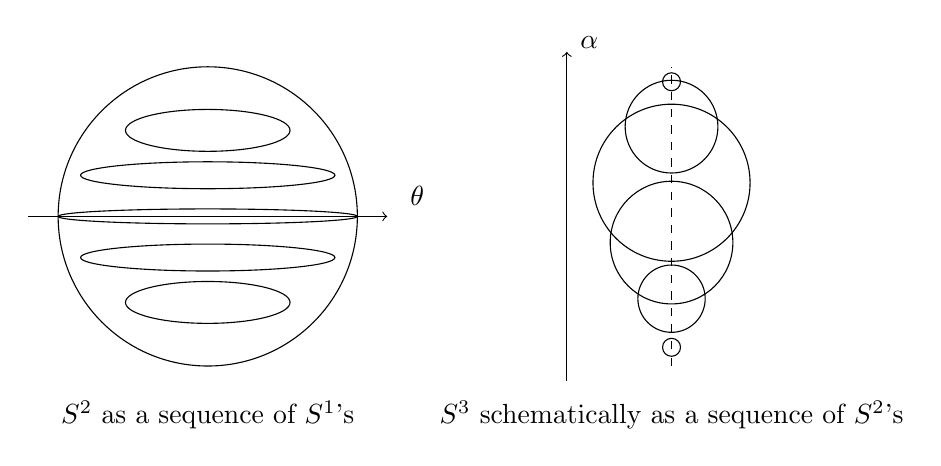
\begin{tikzpicture}[scale=0.95]
\draw (-4,0) circle (2.0);
\draw (-4,1.15) ellipse (1.10 and 0.28);
\draw (-4,0.55) ellipse (1.70 and 0.18);
\draw (-4,0.00) ellipse (2.00 and 0.10);
\draw (-4,-0.55) ellipse (1.70 and 0.18);
\draw (-4,-1.15) ellipse (1.10 and 0.28);
\draw[->] (-6.4,0) -- (-1.6,0);
\node at (-1.20,0.28) {$\theta$};
\node at (-4,-2.65) {$S^2$ as a sequence of $S^1$'s};

\draw[dashed] (2.2,-2.0) -- (2.2,2.0);
\draw (2.2,-1.75) circle (0.12);
\draw (2.2,-1.10) circle (0.45);
\draw (2.2,-0.35) circle (0.82);
\draw (2.2,0.45) circle (1.05);
\draw (2.2,1.20) circle (0.62);
\draw (2.2,1.80) circle (0.12);
\draw[->] (0.8,-2.2) -- (0.8,2.2);
\node at (1.10,2.32) {$\alpha$};
\node at (2.2,-2.65) {$S^3$ schematically as a sequence of $S^2$'s};
\end{tikzpicture}
}%
\caption{The lecture's constructive picture: a two-sphere built from one-spheres whose radius grows and shrinks, and a three-sphere built the same way one dimension higher.}
\end{figure}

This is the real geometric backbone of the lecture. Once the pattern is seen, the four-dimensional embedding picture becomes unnecessary. The geometry is already in the metric.

It also becomes clear why the sphere is special. We could replace \(\sin^2\theta\) by some other function that vanishes at both ends and still obtain a smooth closed surface, but then the resulting geometry would not be uniform. An ellipsoid, for example, is perfectly smooth, but it is not homogeneous; its curvature varies from place to place. The sphere is special precisely because every point looks the same.

\section{From a Static Three-Sphere to a Positively Curved FRW Universe}

Once the unit-sphere metric is in hand, the next move is almost embarrassingly simple. To obtain a sphere of fixed radius \(A\), one multiplies the unit metric by \(A^2\):
\begin{equation}
ds^2=A^2\,d\Omega_3^2.
\end{equation}
The square is important. A metric measures squared distances, so the radius must enter as \(A^2\), not as \(A\).

Now the lecture turns from space to spacetime. We no longer consider a static three-sphere of fixed radius, but a three-sphere whose radius varies with time. At this point one must keep the warning sharp: time is not another embedding coordinate. The fact that space is spherical does not mean that spacetime is a higher-dimensional sphere. The cosmological degree of freedom is instead the time-dependent radius \(a(t)\).

The lecture also assumes, as FRW cosmology does, that the metric has no mixed space-time terms such as \(dtdx\). With that assumption the positively curved FRW spacetime metric is
\begin{equation}
d\tau^2=dt^2-a(t)^2\,d\Omega_3^2.
\end{equation}
Equivalently,
\begin{equation}
d\tau^2=dt^2-a(t)^2\left(d\alpha^2+\sin^2\alpha\,d\Omega_2^2\right).
\end{equation}

This is the first genuinely cosmological metric of the lecture. It describes a universe whose spatial slices are three-spheres, and whose size changes with time. One may think of the Big Bang, in this language, as a three-sphere that begins very small and then expands.

To make the geometry intelligible from the inside, Susskind chooses one pole and places us there. That does not make us special; it merely chooses coordinates convenient for an observer. With that choice, \(\alpha\) can be interpreted as a radial coordinate away from us on the unit sphere. It is not a radial distance in kilometers. It is an angular measure, hence dimensionless, but it plays the role of radial distance in the geometry.

\begin{figure}[htbp]
\centering
\resizebox{\linewidth}{!}{%
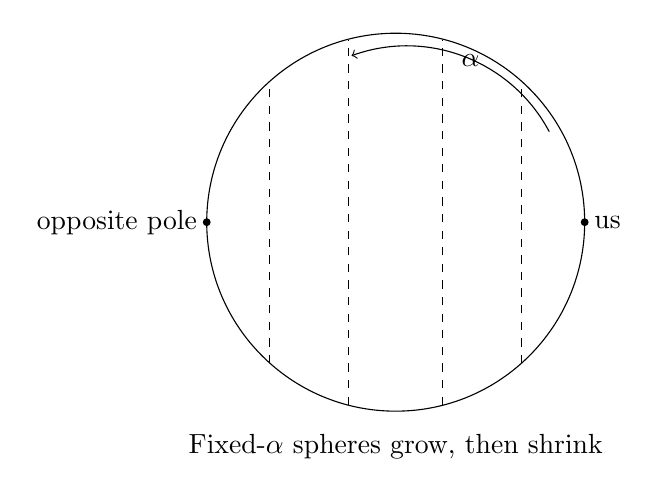
\begin{tikzpicture}[scale=1.0]
\def\R{2.4}
\draw (0,0) circle (\R);
\fill (\R,0) circle (0.05);
\node[right] at (\R,0) {us};
\fill (-\R,0) circle (0.05);
\node[left] at (-\R,0) {opposite pole};

\draw[dashed] (1.6,-1.79) -- (1.6,1.79);
\draw[dashed] (0.6,-2.32) -- (0.6,2.32);
\draw[dashed] (-0.6,-2.32) -- (-0.6,2.32);
\draw[dashed] (-1.6,-1.79) -- (-1.6,1.79);

\draw[->] (1.95,1.15) arc[start angle=28,end angle=110,radius=2.05];
\node at (0.95,2.05) {$\alpha$};

\node at (0,-2.85) {Fixed-\(\alpha\) spheres grow, then shrink};
\end{tikzpicture}
}%
\caption{Observer-centered spherical geometry in two-dimensional cross-section. In three dimensions the fixed-\(\alpha\) surfaces are two-spheres around us: they first grow with distance and then, after a maximum, begin to shrink.}
\end{figure}

In two dimensions the fixed-\(\alpha\) sets are circles around us; in three dimensions they are two-spheres. The striking fact is that as we look farther away, these two-spheres first get larger, then eventually smaller. That is the positive-curvature intuition the lecture will soon turn into an observational statement.

This spacetime geometry is what Susskind calls FRW, following common usage even though one sometimes inserts an \(L\) for Lema\^\i tre. The spherical case is labeled by
\begin{equation}
k=+1.
\end{equation}
At this stage \(k\) is first of all a sign: it means positive \emph{spatial} curvature, not positive spacetime curvature.

\section{Looking Outward: Stereographic Projection and Angular Size}

At this point the lecture deliberately pauses the formalism. A metric by itself is not yet a picture. We want to know what a positively curved space looks like to an astronomer who sits at one point and looks outward. This is why Susskind spends so much time drawing projections: curvature should be translated into something one might see in the sky.

The stereographic projection is the key construction. Take a two-sphere resting on a plane tangent at the south pole. To map a point \(P\) on the sphere to the plane, draw the straight line from the north pole through \(P\), and continue it until it hits the plane. The intersection point is the image \(P'\).

\begin{figure}[htbp]
\centering
\resizebox{\linewidth}{!}{%
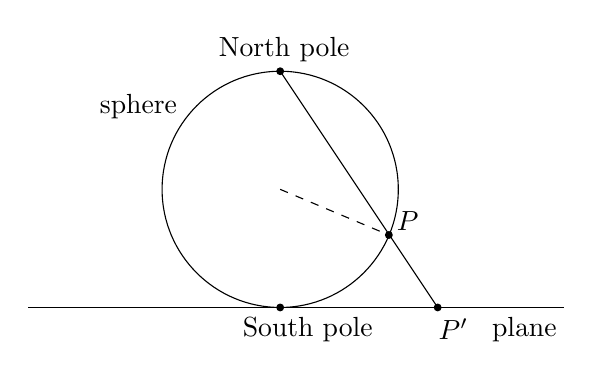
\begin{tikzpicture}[scale=1.0]
\draw (-3.2,0) -- (3.6,0);
\node at (3.10,-0.28) {plane};

\draw (0,1.5) circle (1.5);

\fill (0,3) circle (0.05);
\node at (0.05,3.28) {North pole};

\fill (0,0) circle (0.05);
\node at (0.35,-0.28) {South pole};

\fill (1.38,0.92) circle (0.05);
\node at (1.62,1.10) {$P$};

\fill (2.0,0.0) circle (0.05);
\node at (2.2,-0.28) {$P'$};

\draw (0,3) -- (2,0);
\draw[dashed] (0,1.5) -- (1.38,0.92);

\node at (-1.8,2.55) {sphere};
\end{tikzpicture}
}%
\caption{Stereographic projection from the north pole onto the plane tangent at the south pole. The north pole itself is sent to the point at infinity.}
\end{figure}

This mapping is already telling us something. Near the south pole, where we have placed ourselves, the projection is gentle. But points near the north pole are sent very far away. In fact the north pole itself becomes the point at infinity. Thus the projection of a finite sphere occupies an infinite plane.

Now come the observational consequences. If equal ``continents'' are placed farther and farther away on the sphere, their stereographic images become larger and larger. Translating that into astronomy: in a positively curved space, a standard ruler at fixed distance subtends a larger angle than it would in flat space. Distant objects look too big. This is not merely a cartographic curiosity; it is the operational signature of positive curvature.

One can say the same thing in the language of triangles. On a positively curved surface, the sum of the angles of a triangle is greater than \(180^\circ\). The sky remembers that. A curved geometry changes the relation between physical size, distance, and angular size.

The lecture also stresses a practical point. Angle alone is not enough. One needs both angular size and distance, together with some reason to believe the object's actual size is known well enough for it to act as a standard ruler. In that sense the astronomer becomes a surveyor, measuring large triangles in the sky.

\subsection{Question \& Answer}

\paragraph{Question.} Why do circles stay circles, and what exactly does conformal mean here?

\paragraph{Answer.} Stereographic projection has two different virtues. First, circles on the sphere project to circles in the plane, with straight lines understood as circles of infinite radius. That is a special property of this projection. Second, it is conformal: it preserves angles. Conformal does \emph{not} mean that sizes are preserved. It means that sufficiently small shapes keep their local shape because the angles between directions are unchanged. Thus a small continent keeps the right shape while acquiring the wrong scale. The Mercator projection has the second property as well; stereographic projection has both.

A related warning belongs here. Because the projection stretches distances differently in different regions, signal propagation drawn on the map may appear to speed up or slow down across the page. That is a property of the projection, not a physical change in the speed of light.

\section{Negative Curvature, the Hyperbolic Metric, and the Disk Picture}

Having said, in effect, ``that is about everything we need to know about spheres,'' the lecture pivots to a new homogeneous geometry. It is not literally the opposite of a sphere, but it is the standard example of uniform negative curvature.

Susskind's route is important. He does not begin with the picture. He begins with the metric, by analogy with the sphere:
\begin{equation}
d\mathcal H_n^2=d\alpha^2+\sinh^2\alpha\,d\Omega_{n-1}^2.
\end{equation}
Notice carefully what changes and what does not. The angular factor \(d\Omega_{n-1}^2\) is still the metric of the ordinary unit sphere of one lower dimension. What changes is the growth law of its radius. We replace \(\sin\alpha\) by \(\sinh\alpha\).

The hyperbolic sine is
\begin{equation}
\sinh\alpha=\frac{e^\alpha-e^{-\alpha}}{2}.
\end{equation}
The student correction in the lecture matters: the minus sign is the correct one. Also, \(\alpha\) is no longer an angle running from one pole to another. In the hyperbolic case it runs from
\begin{equation}
0\leq \alpha < \infty.
\end{equation}

This single change is the whole story geometrically. For the sphere, \(\sin\alpha\) starts at zero, rises, and returns to zero. For negative curvature, \(\sinh\alpha\) starts at zero and then keeps growing. So the spheres around us do not first grow and then shrink. They grow without bound, and indeed exponentially for large \(\alpha\).

In three spatial dimensions we therefore write
\begin{equation}
d\mathcal H_3^2=d\alpha^2+\sinh^2\alpha\,d\Omega_2^2.
\end{equation}
Only after this algebraic setup is in place does the lecture turn to the picture.

\begin{figure}[htbp]
\centering
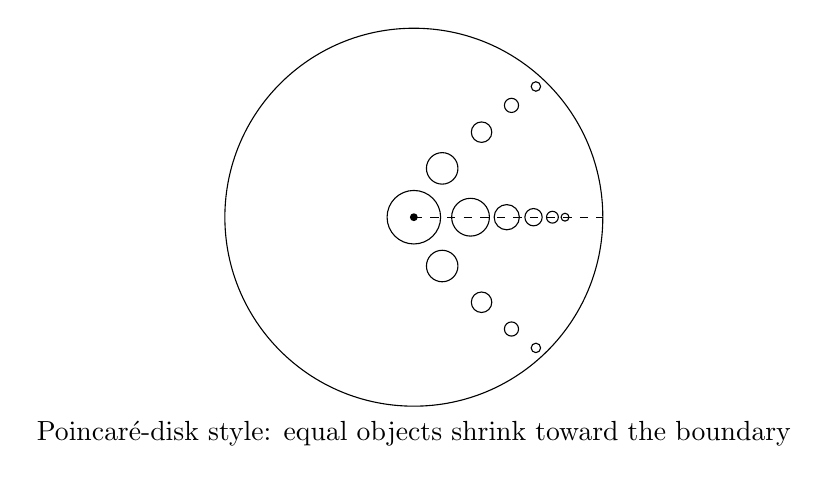
\begin{tikzpicture}[scale=1.0]
\draw (0,0) circle (2.4);
\fill (0,0) circle (0.05);

\draw (0.00,0.00) circle (0.34);
\draw (0.72,0.00) circle (0.24);
\draw (1.18,0.00) circle (0.16);
\draw (1.52,0.00) circle (0.11);
\draw (1.76,0.00) circle (0.075);
\draw (1.92,0.00) circle (0.05);

\draw (0.36,0.62) circle (0.20);
\draw (0.86,1.08) circle (0.13);
\draw (1.24,1.42) circle (0.09);
\draw (1.55,1.66) circle (0.06);

\draw (0.36,-0.62) circle (0.20);
\draw (0.86,-1.08) circle (0.13);
\draw (1.24,-1.42) circle (0.09);
\draw (1.55,-1.66) circle (0.06);

\draw[dashed] (0,0) -- (2.4,0);
\node at (0,-2.75) {Poincar\'e-disk style: equal objects shrink toward the boundary};
\end{tikzpicture}
\caption{A schematic disk picture for negative curvature. The boundary looks finite in the drawing, but the intrinsic distance to it is infinite.}
\end{figure}

The lecture likes to compare this with the stereographic projection of the sphere. There the page looked infinite, but the actual spherical distance was finite. Here the page looks finite, but the actual hyperbolic distance is infinite. Equal objects appear smaller and smaller as they approach the boundary. The drawing is deceptive in exactly the opposite way.

This is why distant objects in a negatively curved universe look too small relative to flat space. A standard ruler at fixed distance subtends too small an angle. Again the geometry has become an observational statement.

Only after the disk picture has been understood does the lecture write the cosmological spacetime metric:
\begin{equation}
d\tau^2=dt^2-a(t)^2\,d\mathcal H_3^2.
\end{equation}
This is the negatively curved FRW universe, often described in the lecture as the infinite FRW case. Its sign label is
\begin{equation}
k=-1.
\end{equation}

Two more geometric remarks from the lecture should be preserved. First, this negatively curved space is still homogeneous. The drawing looks wildly inhomogeneous because the tiles near the edge are tiny, but any observer moved to another location sees the same intrinsic geometry. Second, one can draw small patches of negative curvature as saddle-shaped surfaces, but only locally. There is no global embedding of the entire hyperbolic space as a nice ordinary surface in Euclidean three-space.

\subsection{Question \& Answer}

\paragraph{Question.} Why does a finite-looking disk represent an infinite homogeneous space?

\paragraph{Answer.} Because the Euclidean size in the drawing is not the intrinsic size in the metric. The little tiles or continents near the edge are geometrically the same size as those near the center; only their \emph{pictures} are smaller. If one measures distance by counting equal geometric tiles, one crosses infinitely many before reaching the boundary. The boundary therefore lies at infinite distance even though it looks finite on the page. Homogeneity survives because every tile is intrinsically like every other one, and the isometries of the space move one location into another without changing the geometry.

\section{The Flat Limit and the Three FRW Cases}

Only once the positively and negatively curved cases are on the table does the lecture turn to the intermediate case. Flat space is the boundary between them. One may think of it as a limit if one likes, but Susskind eventually says not to fuss over that. It is simply flat Euclidean space.

The corresponding FRW metric is
\begin{equation}
d\tau^2=dt^2-a(t)^2\left(dx^2+dy^2+dz^2\right).
\end{equation}
Its label is
\begin{equation}
k=0.
\end{equation}

At this point the three classical homogeneous cosmologies can be stated cleanly:
\begin{align}
k=+1 &: \text{space is spherical and positively curved}, \\
k=0 &: \text{space is flat}, \\
k=-1 &: \text{space is hyperbolic with negative curvature}.
\end{align}

This is a regrouping moment in the lecture, not yet the final payoff. We have built the three geometries, understood how they distort angular sizes, and attached the sign labels \(k=+1,0,-1\). Only now are we ready to return to the earlier cosmological equations and ask what Einstein has to do with them.

\section{Newtonian Cosmology Recalled, Einstein Cosmology Interpreted}

After the break Susskind does not jump straight to general relativity. He backs up. That is important to the rhythm of the argument: the old Newtonian constant must be put back on the table before its geometric meaning can be explained.

The board at the transition still carries a fragment of the flat FRW metric:

\begin{figure}[htbp]
\centering

\includegraphics[width=0.72\textwidth]{lecture_05_figure_02.png}
\caption{Flat-space metric fragment on the board, carried into the transition back from the break.}
\end{figure}

The screenshot only certifies the visible spatial piece \(dx^2+dy^2+dz^2\), but that is enough to witness the board continuity: the lecture is now moving from the three FRW metrics toward general relativity.

The Newtonian recap is brief and disciplined. Put ourselves at the center. Consider a galaxy at distance \(r(t)\) moving away according to the Hubble flow. By Newton's shell theorem, only the mass inside the sphere of radius \(r\) contributes to the force on that galaxy. Writing the Newtonian energy equation per unit mass,
\begin{align}
\frac{1}{2}\dot r^{\,2}-\frac{GM(r)}{r} &= E, \\
M(r) &= \frac{4\pi}{3}r^3\rho.
\end{align}
For a comoving galaxy we may write
\begin{equation}
r(t)=a(t)\chi,
\end{equation}
with \(\chi\) fixed. Then \(\dot r=\dot a\,\chi\), and after dividing through by \(a^2\chi^2\) one arrives at the Newtonian cosmology equation in the form
\begin{equation}
\left(\frac{\dot a}{a}\right)^2=\frac{8\pi G}{3}\rho-\frac{k}{a^2},
\end{equation}
where the last term packages the previously omitted constant total-energy contribution. The knife-edge case studied earlier corresponds to setting that constant to zero, that is, exactly the escape-velocity case.

The lecture also reinstates the density scalings that accompany the matter content:
\begin{align}
\rho_m &\propto a^{-3}, &
\rho_r &\propto a^{-4}, &
\rho_{\mathrm{vac}} &= \text{const.}
\end{align}
and, as before, pressure is written as
\begin{equation}
p=w\rho,
\end{equation}
with the familiar cases
\begin{equation}
w=0,\qquad w=\frac{1}{3},\qquad w=-1
\end{equation}
for matter, radiation, and vacuum energy.

Only now does the lecture turn to Einstein's field equations. The board writes a compressed version, and the top-to-bottom staging is itself part of the rhetoric: first the general field equation, then the \(00\) component that cosmology actually needs.

\begin{figure}[htbp]
\centering

\includegraphics[width=0.62\textwidth]{lecture_05_figure_05.png}
\caption{Einstein equation on the top line and its \(00\) component below it.}
\end{figure}

The board image does not show the factor \(\tfrac12\) multiplying \(g^{\mu\nu}R\) clearly, but the lecture later acknowledges that a half belongs there. We therefore write the cleaned form while preserving the lecture's normalization:
\begin{equation}
R^{\mu\nu}-\frac{1}{2}g^{\mu\nu}R=4\pi G\,T^{\mu\nu}.
\end{equation}
The \(00\)-component becomes
\begin{equation}
R^{00}-\frac{1}{2}g^{00}R=4\pi G\,\rho.
\end{equation}

The left-hand side is geometry, now spacetime geometry rather than merely spatial geometry. The right-hand side is matter, more precisely the energy-momentum tensor. The lecture also reminds us that the other components of \(T^{\mu\nu}\) need not vanish. In particular, the space-space components encode pressure. That is why the equation of state \(p=w\rho\) remains in the story even though the \(00\) equation is the one singled out to determine \(a(t)\).

\subsection{Question \& Answer}

\paragraph{Question.} Why is one Einstein equation enough once FRW symmetry leaves only \(a(t)\) as the unknown?

\paragraph{Answer.} Because by the time we reach Einstein's equations we have already assumed an enormous amount. We have assumed homogeneity. We have assumed isotropy. We have assumed that the spatial slices are of one of the three FRW types. After all of that, the metric contains only one dynamical function, the scale factor \(a(t)\). Many tensor equations remain formally present, but there is only one independent unknown function to solve for. The \(00\) component is the natural choice because \(T^{00}\) is the energy density \(\rho\), so this component most directly ties geometry to the cosmological matter content.

The lecture does not carry out the curvature calculation in detail on the board. Instead it tells us what kind of terms must appear when the FRW metric is substituted into the Einstein tensor.

First, there is a contribution that comes from the fact that the geometry is time dependent. It would be there even if space were flat. This term is proportional to
\begin{equation}
\left(\frac{\dot a}{a}\right)^2.
\end{equation}
It represents spacetime curvature produced purely by the changing scale factor.

Second, there is a contribution that would remain even if the scale factor were frozen. This is the contribution of spatial curvature itself. For a homogeneous space of fixed shape, curvature scales like the inverse radius squared:
\begin{equation}
\text{curvature} \propto \frac{1}{a^2}.
\end{equation}
With the sign convention already prepared by the geometry, that contribution is
\begin{equation}
\frac{k}{a^2}.
\end{equation}
Positive curvature contributes with a plus sign, negative curvature with a minus sign, and flat space with zero.

The lecture's coefficient bookkeeping here is informal and partly self-correcting; Susskind checks the answer against the earlier Newtonian result rather than presenting a polished tensor derivation. The cleaned endpoint is
\begin{equation}
\left(\frac{\dot a}{a}\right)^2+\frac{k}{a^2}=\frac{8\pi G}{3}\rho,
\end{equation}
or equivalently
\begin{equation}
\left(\frac{\dot a}{a}\right)^2=\frac{8\pi G}{3}\rho-\frac{k}{a^2}.
\end{equation}

This is the real destination of the lecture. The same symbol \(k\) is now seen in two lights. From the Newtonian point of view, it classifies the motion: above escape velocity, at escape velocity, or below escape velocity. From the Einstein point of view, it classifies the shape of space itself: hyperbolic, flat, or spherical.

There is one final normalization subtlety that the lecture brings out in discussion. In the spherical and hyperbolic cases there is a natural curvature radius, so one may choose \(a(t)\) so that \(k=\pm 1\). In the flat case there is no distinguished spatial radius, so \(a(t)\) may be rescaled without changing the statement \(k=0\). Thus the three values \(k=+1,0,-1\) are best thought of as a sign classification once the natural curvature scale has been absorbed into \(a(t)\).

This is why general relativity does not simply replace the earlier Newtonian cosmology. It explains it. The old integration constant was already measuring something real; Einstein tells us that what it was measuring was the curvature of space.

\section{Summary}

The lecture unfolds in a very deliberate order. We begin with spheres, not because cosmology has become geometry for its own sake, but because homogeneous cosmology needs a precise language for homogeneous spaces. The recursive construction of \(S^1\), \(S^2\), and \(S^3\) then becomes the spatial part of the FRW metrics once the fixed radius is promoted to \(a(t)\).

The long visual detour is equally essential. Positive curvature makes standard rulers look too large, negative curvature makes them look too small, and stereographic or disk pictures teach us how to think from the observer's point of view. Only after that does the Einstein bridge become intelligible. The final Friedmann equation contains exactly the two geometric ingredients the lecture has prepared us for: the time-variation term \((\dot a/a)^2\) and the spatial-curvature term \(k/a^2\). The sign \(k\) is therefore both a dynamical classifier and a statement about the shape of space.
